\documentclass[journal]{IEEEtran}
\usepackage{cite}
\usepackage{amsmath,amssymb,amsfonts,amsthm}
\usepackage{graphicx}
\usepackage{algorithm}
\usepackage{algorithmic}
\usepackage{booktabs}
\usepackage{xcolor}
\usepackage{tikz}
\usetikzlibrary{positioning,arrows.meta}
\usepackage[hidelinks]{hyperref}
\newtheorem{proposition}{Proposition}

\begin{document}

\title{IMBANG: Balancing DDoS Mitigation and Service Outages with Safety-Spanning Group-Relative Policy Optimisation}

\author{Muntakimur~Rahaman, Azwan~Mahmud, Abdellah~Chehri, and~Bijan~Raahemi%
\thanks{M. Rahaman and A. Mahmud are with the Faculty of Artificial Intelligence and Engineering, Multimedia University, Cyberjaya 63100, Selangor, Malaysia (e-mail: muntakimur.rahaman@student.mmu.edu.my; azwan.mahmud@mmu.edu.my).}%
\thanks{A. Chehri is with the Department of Mathematics and Computer Science, Royal Military College of Canada, Kingston, ON K7K 7B4, Canada (e-mail: abdellah.chehri@rmc-cmr.ca).}%
\thanks{B. Raahemi is with the Telfer School of Management and the Digital Transformation and Innovation Program, University of Ottawa, Ottawa, ON K1N 6N5, Canada (e-mail: braahemi@uottawa.ca).}}

\markboth{IEEE Networking Letters}{IMBANG: Balancing DDoS Mitigation and Service Outages}

\maketitle

\begin{abstract}
Sentinel combines PPO, a co-evolving attacker, and symbolic shielding for DDoS mitigation, yet severe outages persist under floods. We replace this loop with critic-free Group Relative Policy Optimization (GRPO) and show that group centring removes the marginal influence of an outage penalty whenever all rollouts share the same outage count. Naive GRPO reduces leakage while increasing outages. IMBANG adds one guaranteed no-less-safe rollout per group with an outage budget. Over ten seeds, IMBANG achieves higher composite scores than Sentinel in all eight scenarios, reduces severe outages by 57\%, and meets the outage budget in nine seeds.
\end{abstract}

\begin{IEEEkeywords}
DDoS mitigation, 6G security, safe reinforcement learning, group-relative policy optimisation.
\end{IEEEkeywords}

% ===========================================================================
\section{Introduction}
% ===========================================================================
\IEEEPARstart{Z}{ero-touch} 6G management expects edge controllers to absorb volumetric DDoS floods in closed loop~\cite{benzaid2020zsm,liyanage2023oran}. Such a controller must discard hostile traffic without starving legitimate users: a filter that is too aggressive causes the outage it was meant to prevent~\cite{guo2020xai6g}. Deep reinforcement learning has been applied to throttling, SDN flow control and per-host drop policies~\cite{malialis2015distributed,liu2018drlddos,simpson2020perhost}. Sentinel~\cite{alfatemi2026sentinel} is the most advanced recent design. It trains its agent with Proximal Policy Optimization (PPO)~\cite{schulman2017ppo} against a co-evolving attacker and inserts a symbolic shield~\cite{alshiekh2018shielding} between the agent and the network. Its authors report that training deteriorates late in every seed and that severe outages persist under heavy floods.

Group Relative Policy Optimization (GRPO)~\cite{shao2024deepseekmath} looks like a natural successor. It compares several rollouts started from one state, so neither a value network nor a learned opponent is needed. In a simulator these rollouts can share one realisation of the traffic process~\cite{ng2000pegasus}, so that they differ only in the defender's actions. We find, however, that GRPO defenders leak less attack traffic than Sentinel but cause \emph{more} severe outages. The reason is structural. A cost that every member of a group incurs is removed by the group mean, mirroring the gradient starvation of binary-reward GRPO~\cite{nie2026starvation,yu2025dapo}. Separate normalisation of the cost channel, as in Constrained GRPO~\cite{girgis2026cgrpo}, does not help when that channel has no variance within a group. Injecting reference samples into groups stabilises language-model training~\cite{yan2025luffy,armor2026}, but no safe direction is available in that setting. Table~\ref{tab:related} summarises how these approaches treat the outage constraint.

\begin{table}[t]
\centering
\caption{Treatment of the Outage Constraint by Related Approaches}
\label{tab:related}
\setlength{\tabcolsep}{2.5pt}
\resizebox{\columnwidth}{!}{%
\begin{tabular}{@{}lcccc@{}}
\toprule
 & Critic- & No learned & Outage & Cost signal when all \\
Approach & free & attacker & budget & members violate \\
\midrule
Sentinel~\cite{alfatemi2026sentinel} & -- & -- & -- & n/a (critic) \\
PPO-Lagrangian / CPO~\cite{achiam2017cpo} & -- & \checkmark & \checkmark & n/a (critic) \\
GRPO~\cite{shao2024deepseekmath} with penalty & \checkmark & \checkmark & \checkmark & -- \\
Constrained GRPO~\cite{girgis2026cgrpo} & \checkmark & \checkmark & \checkmark & -- \\
Sign advantage~\cite{nie2026starvation} & \checkmark & \checkmark & -- & fixed reference \\
\textbf{IMBANG} & \checkmark & \checkmark & \checkmark & \checkmark\ (safe member) \\
\bottomrule
\end{tabular}}
\end{table}

This letter makes three key contributions. First, it derives this \emph{constraint-cancellation} effect and validates it on 80 trained checkpoints (Section~\ref{sec:mechanism}). Second, it proposes IMBANG (\textbf{I}nterpretable, \textbf{M}onotone-safe, \textbf{B}udgeted, \textbf{A}dversary-free, \textbf{N}euro-symbolic \textbf{G}RPO), whose \emph{safe-side member} keeps every group straddling the outage boundary with a proven monotonicity guarantee (Section~\ref{sec:method}). Third, it benchmarks IMBANG against Sentinel's released checkpoints, a compute-matched PPO baseline, Constrained GRPO and the simplest alternative remedies over ten seeds (Section~\ref{sec:eval}).

% ===========================================================================
\section{System Model}
\label{sec:system}
% ===========================================================================
\begin{figure}[t]
\centering
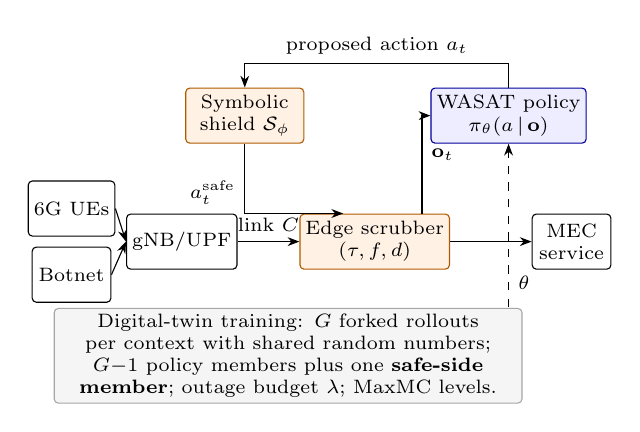
\begin{tikzpicture}[font=\scriptsize, >={Stealth[length=1.5mm]},
  box/.style={draw, rounded corners=1.5pt, align=center, inner sep=2pt, minimum height=7mm, fill=white},
  ag/.style={box, fill=blue!7, draw=blue!60!black}, sy/.style={box, fill=orange!10, draw=orange!70!black},
  tr/.style={box, fill=gray!8, draw=gray!70}]
\node[box, minimum width=10mm] (ue) at (0, 0.42) {6G UEs};
\node[box, minimum width=10mm] (bot) at (0,-0.42) {Botnet};
\node[box, minimum width=11mm] (gnb) at (1.4, 0) {gNB/UPF};
\node[sy, minimum width=17mm] (scr) at (3.85, 0) {Edge scrubber\\$(\tau,f,d)$};
\node[box, minimum width=10mm] (mec) at (6.35, 0) {MEC\\service};
\node[ag, minimum width=19mm] (pol) at (5.55, 1.6) {WASAT policy\\$\pi_\theta(a\,|\,\mathbf{o})$};
\node[sy, minimum width=15mm] (sh) at (2.2, 1.6) {Symbolic\\shield $\mathcal{S}_\phi$};
\node[tr, text width=58mm] (twin) at (2.75,-1.45) {Digital-twin training: $G$ forked rollouts per context with shared random numbers; $G{-}1$ policy members plus one \textbf{safe-side member}; outage budget $\lambda$; MaxMC levels.};
\draw[->] (ue.east) -- (gnb.west);
\draw[->] (bot.east) -- (gnb.west);
\draw[->] (gnb) -- node[above]{link $C$} (scr);
\draw[->] (scr) -- (mec);
\draw[->] ([xshift=6mm]scr.north) |- node[pos=0.3, right]{$\mathbf{o}_t$} (pol.west);
\draw[->] (pol.north) -- ++(0,0.3) -| node[pos=0.25, above]{proposed action $a_t$} (sh.north);
\draw[->] (sh.south) |- node[pos=0.35, left]{$a^{\mathrm{safe}}_t$} ([xshift=-4mm]scr.north);
\draw[->, dashed] (twin.east -| pol.south) ++(0,0.62) -- node[pos=0.15, right]{$\theta$} (pol.south);
\end{tikzpicture}
\caption{System model. At the 6G edge, a learned filtering policy configures a scrubber placed in front of the MEC service, and every proposal passes through a symbolic shield. The policy is trained in a digital twin using safety-spanning rollout groups.}
\label{fig:system}
\end{figure}

We use the system model of~\cite{alfatemi2026sentinel}, shown in Fig.~\ref{fig:system}. User equipment and a botnet share a gNB/UPF link that feeds an edge scrubber placed in front of a multi-access edge computing (MEC) service. In each control window the learned policy proposes a filtering action from aggregate telemetry, the symbolic shield repairs any unsafe proposal, and the scrubber applies the result. The policy is trained offline in a digital twin of this loop (Section~\ref{sec:method}).

The edge link has capacity $C$ and carries benign traffic $L_t\sim\mathrm{Poisson}(\mu)$ and attack traffic $A_t=1.5\,C\,i_t$. The attack belongs to a family in $\{\mathrm{SYN},\mathrm{UDP},\mathrm{HTTP},\mathrm{ICMP},\mathrm{mixed}\}$, with intensity $i_t\in[0,1]$ and a mutation level $m_t$ that weakens filter matching; flash crowds may inflate $L_t$ up to fourfold. ICMP is withheld from training. In each control window the defender observes twelve aggregate indicators $\mathbf{o}_t\in[0,1]^{12}$, measured on served traffic. It then sets a load threshold $\tau_t$, a filtering focus $f_t\in\{\mathrm{SrcIP},\mathrm{Proto},\mathrm{Size}\}$ and a drop probability $d_t$. With match effectiveness $\eta=\eta_{kf}(1-m_t/2)$, the share of benign traffic lost to filtering is
\begin{equation}
\mathrm{CD}_t = 0.4\,d_t(1-\eta)\,\alpha(\tau_t) + 0.2\,[L_t-C\tau_t]^+/L_t ,
\label{eq:cd}
\end{equation}
where $\alpha(\tau)$ is the fraction of offered load above the threshold. Service quality is $\mathrm{SQ}_t=\rho_t(1-\mathrm{CD}_t)$, with congestion factor $\rho_t=\min\{1,C/(L_t+A_t)\}$. A window with $\mathrm{SQ}_t<0.5$ is a \emph{severe outage}. The operator scores each window with Sentinel's benchmark,
$b_t=\mathrm{SQ}_t-\mathrm{leak}_t-0.5\,\mathbf{1}[\mathrm{SQ}_t<0.5]-0.25\,\mathbf{1}[\mathrm{SQ}_t<0.75]$,
where $\mathrm{leak}_t$ is the share of attack traffic delivered. A symbolic shield $\mathcal{S}_\phi$ edits unsafe actions through per-coordinate clamps. The defender solves
\begin{equation}
\max_\theta\ \mathbb{E}_{\pi_\theta}\Big[\textstyle\sum_t b_t\Big]\quad\text{s.t.}\quad \sigma(\pi_\theta)\le\kappa=0.05 ,
\label{eq:cpomdp}
\end{equation}
where $\sigma$ is the severe-outage frequency on the operator's validation scenarios. The budget $\kappa$ was fixed before the ten-seed experiments. The traffic, observation and service models, \eqref{eq:cd}, the score $b_t$ and the shield are taken unchanged from~\cite{alfatemi2026sentinel}. Our new elements are the budgeted formulation~\eqref{eq:cpomdp}, the cancellation result (Proposition~\ref{prop:cancel}) and the safe-side construction with its guarantee (Proposition~\ref{prop:safe}).

% ===========================================================================
\section{Constraint Cancellation}
\label{sec:mechanism}
% ===========================================================================
GRPO copies each training context into $G$ members that replay the same traffic. Member $g$ collects objective $O_g=\sum_h b_h$ and outage count $K_g$ over $H$ windows. With a Lagrange multiplier $\lambda$, the return is $R_g=O_g-\lambda K_g$ and the advantage is $\hat A_g=(R_g-\bar R)/s_R$, normalised by the group mean and standard deviation.

\begin{proposition}\label{prop:cancel}
If $K_g\equiv K$ within a group, then $\hat A_g$ is identical for all $\lambda\ge0$. The same holds for channel-wise normalisation $\hat A_g=\mathrm{z}(O)_g-\lambda\,\mathrm{z}(K)_g$~\cite{girgis2026cgrpo} with $\mathrm{z}(K)_g:=0$ when $s_K=0$.
\end{proposition}
\begin{proof}
$R_g-\bar R=O_g-\bar O$ and $s_R=s_O$; channel-wise, $s_K=0$ gives $\mathrm{z}(K)\equiv0$.
\end{proof}

The constraint therefore acts only through groups whose members disagree about the outage count; we call their share the \emph{span rate}. Leakage, being continuous, almost always varies. Under a full-intensity flood ($\rho_t\approx0.56$), a window becomes a severe outage once $\mathrm{CD}_t>1-0.5/\rho_t\approx0.10$. This threshold moves with the intensity, which is hard to observe once the link saturates. As GRPO sharpens its policy, whole groups fall beyond the threshold, and only the leakage term keeps steering the update.

Fig.~\ref{fig:mech} tests this explanation on 80 trained checkpoints under overload. The span rate grows with the within-group spread of the drop action ($r=0.91$), and checkpoints with a lower span rate suffer more severe outages ($r=-0.61$). Plain GRPO keeps a drop spread of 0.05, spans 47\% of groups and causes severe outages in 76\% of windows. PPO and Sentinel keep a spread above 0.21 and span every group.

\begin{figure}[t]
\centering
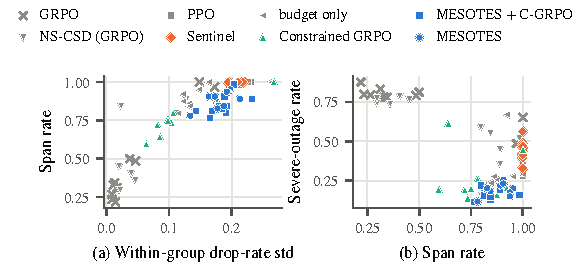
\includegraphics[width=\columnwidth]{figures/mechanism.pdf}
\caption{Constraint cancellation under full-intensity floods (80 checkpoints, $G=8$ members sharing traffic). (a) The span rate increases with the within-group spread of the drop action. (b) A lower span rate coincides with more severe outages.}
\label{fig:mech}
\end{figure}

% ===========================================================================
\section{IMBANG}
\label{sec:method}
% ===========================================================================
IMBANG reserves one \emph{safe-side member} per group. At each window it takes the policy's sample $(\tau,f,d)$, draws $u\sim\mathcal{U}(0.2,0.8)$ once per rollout, and executes $\tilde d=u\,d$, $\tilde\tau=\tau+(1-u)(1-\tau)$ and $\tilde f=f$.

\begin{proposition}\label{prop:safe}
For identical observations and traffic, the safe-side member's collateral damage after shielding never exceeds that of the policy member, so it never incurs more severe outages.
\end{proposition}
\begin{proof}
By~\eqref{eq:cd}, $\mathrm{CD}$ is non-decreasing in $d$ and non-increasing in $\tau$; $\eta$ is unchanged because $f$ is. Each shield rule is a per-coordinate $\min$ or $\max$ triggered by $(\mathbf{o}_t,f)$ only, so it preserves $\tilde d\le d$ and $\tilde\tau\ge\tau$. As $\rho_t$ does not depend on the action, $\mathrm{SQ}$ keeps the same order.
\end{proof}

Hence, whenever the sampled actions cause outages that a gentler filter would avoid, the safe-side member supplies the cost variance that Prop.~\ref{prop:cancel} shows to be necessary. The policy learns from it only through $-c\,[\hat A]^+\log\pi_\theta(\tilde a\,|\,\mathbf{o})$, that is, only when the member outperformed its group. The guarantee holds at every intensity, so IMBANG never needs to locate the threshold. Three further components complete the method:
\begin{itemize}
\item $\lambda$ follows dual ascent on the validation outage rate, $\lambda\leftarrow[\lambda+\eta_\lambda(\hat\sigma-\kappa)]^+$.
\item The deployed checkpoint is selected feasibility first.
\item Training contexts come from 360 discrete attack levels, prioritised by the MaxMC regret estimate~\cite{jiang2021robustplr,jiang2021plr} rather than by a learned attacker.
\end{itemize}
All GRPO variants share the remaining machinery: archive elites, shield probes, a KL anchor to the best validated checkpoint, and Sentinel's two-layer network trained without a critic. Algorithm~\ref{alg:imbang} summarises one training iteration.

\begin{algorithm}[t]
\caption{One IMBANG training iteration}
\label{alg:imbang}
\small
\begin{algorithmic}[1]
\STATE Sample $B$ levels by MaxMC priority; warm up; fork each into $G$ members sharing one traffic realisation
\STATE Assign policy samples, archive elite, shield probes and the safe-side member
\STATE Roll out $H$ windows through $\mathcal{S}_\phi$; form $R_g=O_g-\lambda K_g$ and group advantages $\hat A_g$
\STATE Update $\theta$ with the clipped surrogate on policy members, the $[\hat A]^+$-weighted likelihood on the safe member and the elite, and a KL term to the current champion
\STATE Every $K$ iterations: validate, update $\lambda$, select the champion feasibility first, and refresh the MaxMC regrets
\end{algorithmic}
\end{algorithm}

\textbf{Implementation.} Each run performs 500 iterations with $B=32$ contexts, $G=8$ members, horizon $H=8$, up to 40 warm-up windows and a discovery step every $K=20$ iterations. Optimisation uses Adam with learning rate $3\times10^{-4}$, clipping 0.2, four epochs, a KL weight of 0.02, an elite weight of 0.5 and an entropy weight of 0.005. The multiplier step is $\eta_\lambda=4$ per validation round, and the validation battery contains benign, mild, strong and chaos traffic but no ICMP, so that ICMP remains unseen until testing.

% ===========================================================================
\section{Results and Discussion}
\label{sec:eval}
% ===========================================================================
We re-implemented Sentinel's public simulator and shield~\cite{sentinelcode} in batched form. Unit tests show agreement with the reference code to within $10^{-5}$, and Sentinel's released checkpoints reproduce its published strong-attack results (0.519/0.815/78.2 against 0.519/0.815/75.0 for quality, leakage and severe outages).

\textbf{Protocols.} We compare Sentinel's ten released checkpoints (seeds 42--51) with defenders trained on the same seeds. Protocol~B covers eight attack scenarios, four of them held-out stress tests, with 20 episodes of 100 windows each. Protocol~A replays the attacker that Sentinel trained for each seed, which is a transfer test for IMBANG. Protocol~C is a cross-entropy red team that searches the whole scenario space, ICMP included. All comparisons are paired by seed and traffic. We use paired $t$-tests with Holm correction and Wilcoxon tests.

\begin{table}[t]
\centering
\caption{Protocol B over 10 Seeds: Composite Score ($\uparrow$) and Severe Outages per 500 Windows ($\downarrow$)}
\label{tab:main}
\setlength{\tabcolsep}{2.4pt}
\resizebox{\columnwidth}{!}{%
\begin{tabular}{@{}lcccccc@{}}
\toprule
 & \multicolumn{3}{c}{Composite score} & \multicolumn{3}{c}{Severe outages} \\
\cmidrule(lr){2-4}\cmidrule(l){5-7}
Scenario & Sentinel & C-GRPO & IMBANG & Sentinel & C-GRPO & IMBANG \\
\midrule
Mild & 0.009 & \textbf{0.053} & 0.040\textsuperscript{\dag} & \textbf{0.0} & \textbf{0.0} & \textbf{0.0} \\
Strong & -0.746 & -0.612 & \textbf{-0.583}\textsuperscript{\dag} & 155.2 & 85.9 & \textbf{38.9} \\
Chaos/flash & -0.169 & \textbf{-0.114} & -0.123\textsuperscript{\dag} & 14.1 & 16.8 & \textbf{10.7} \\
ICMP (zero-shot) & -0.474 & -0.474 & \textbf{-0.458}\textsuperscript{\dag} & \textbf{4.6} & 23.3 & 18.0 \\
Pulsing$^\ast$ & -0.303 & -0.228 & \textbf{-0.225}\textsuperscript{\dag} & 60.5 & 37.7 & \textbf{16.1} \\
Polymorphic$^\ast$ & -0.454 & -0.442 & \textbf{-0.430}\textsuperscript{\dag} & 14.9 & 24.0 & \textbf{14.2} \\
Boundary$^\ast$ & 0.003 & \textbf{0.084} & 0.071\textsuperscript{\dag} & \textbf{0.0} & \textbf{0.0} & \textbf{0.0} \\
ICMP-chaos$^\ast$ & -0.299 & \textbf{-0.255} & -0.257\textsuperscript{\dag} & 25.4 & 25.2 & \textbf{20.9} \\
\midrule
Average & -0.304 & -0.248 & -0.246 & 34.4 & 26.6 & 14.8 \\
\bottomrule
\end{tabular}}

\vspace{2pt}
\parbox{\columnwidth}{\scriptsize $^\ast$Held-out stress test. \dag\,IMBANG above Sentinel, paired $t$-test, Holm-corrected, $p<0.05$. Bold: best.}
\end{table}


\textbf{Against Sentinel.} IMBANG scores significantly higher than Sentinel in every attack scenario (Table~\ref{tab:main}); the scenario average is $-0.246$ against $-0.304$ ($p=1.2\times10^{-5}$). Severe outages fall from 34.4 to 14.8 per 500 windows ($p=0.002$) and leakage from 0.876 to 0.839 ($p<10^{-3}$), with service quality unchanged. Against Sentinel's own attackers (Protocol~A), IMBANG also scores higher ($-0.265$ against $-0.332$, $p=0.019$) and leaks less (0.778 against 0.830, $p=0.018$). In five of the eight scenarios it is at least as good as Sentinel on quality, leakage and outages simultaneously; on mild and boundary-rate floods it trades about 0.01 of quality for 4--7 points less leakage. Its red-team worst case improves from $-1.07$ to $-0.72$ ($p=7.2\times10^{-4}$).

\textbf{Operating curve.} Fig.~\ref{fig:intensity} sweeps the flood intensity $i$ with identical traffic for all defenders. Up to $i=0.9$, Sentinel and IMBANG keep severe outages at or below 1.1 per 500 windows, Sentinel marginally lower. As the link saturates, Sentinel's outages climb to 143 per 500 windows at $i=1$, against 84 for Constrained GRPO and 40 for IMBANG, so IMBANG delays and flattens the outage cliff. IMBANG also leaks less than Sentinel at every intensity.

\begin{figure}[t]
\centering
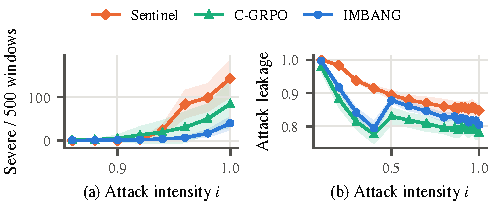
\includegraphics[width=\columnwidth]{figures/intensity.pdf}
\caption{Operating curve over attack intensity (training attack mix, 20 episodes per point, mean and 95\% confidence band over ten seeds). (a) Severe outages near link saturation. (b) Attack leakage.}
\label{fig:intensity}
\end{figure}

\textbf{Budget and remedies.} A PPO baseline given the same 1.34M training windows already improves on Sentinel, which shows the benefit of dropping co-evolution. IMBANG still beats it at equal budget ($+0.030$, $p=2\times10^{-7}$). Table~\ref{tab:ablation} and Fig.~\ref{fig:tradeoff} isolate the safe-side member. A Lagrangian budget alone is met in one seed out of ten even though $\lambda$ rises to about 7.7, as Prop.~\ref{prop:cancel} predicts (Fig.~\ref{fig:dyn}); an entropy bonus or an uncentred cost does not restore feasibility, and Constrained GRPO meets the budget in three seeds. IMBANG meets it in nine with $\lambda\approx0.4$, matching Constrained GRPO's score ($p=0.47$) with fewer outages (14.8 against 26.6) and slightly more leakage (0.839 against 0.820).

\begin{table}[t]
\centering
\caption{Ablation and Alternative Remedies (10 Seeds). Worst: Red-Team Worst Case; Budget: Seeds Meeting $\sigma\le0.05$}
\label{tab:ablation}
\setlength{\tabcolsep}{3pt}
\resizebox{\columnwidth}{!}{%
\begin{tabular}{@{}lcccc@{}}
\toprule
Method & Score $\uparrow$ & Severe $\downarrow$ & Worst $\uparrow$ & Budget \\
\midrule
Sentinel~\cite{alfatemi2026sentinel} & -0.304 & 34.4 & -1.07 & -- \\
PPO + shield (equal budget) & -0.276 & 19.6 & -0.79 & -- \\
GRPO, no budget & -0.250 & 91.5 & -1.07 & -- \\
GRPO + budget & -0.253 & 36.5 & -0.87 & 1/10 \\
\;\; + entropy bonus $\times6$ & -0.249 & 33.8 & -0.85 & 0/10 \\
\;\; + uncentred cost & -0.251 & 34.7 & -0.87 & 1/10 \\
C-GRPO~\cite{girgis2026cgrpo} & -0.248 & 26.6 & -0.80 & 3/10 \\
\textbf{MIZAN} & -0.246 & 14.8 & -0.72 & 9/10 \\
MIZAN + C-GRPO normalisation & -0.247 & 12.1 & -0.71 & 7/10 \\
\bottomrule
\end{tabular}}
\end{table}


\begin{figure}[t]
\centering
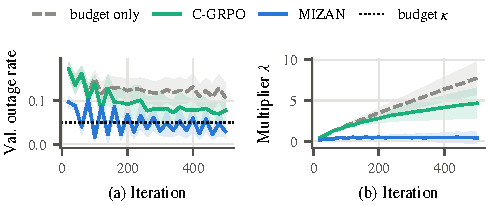
\includegraphics[width=\columnwidth]{figures/dynamics.pdf}
\caption{Training dynamics (mean and 95\% confidence band over ten seeds). (a) Validation outage rate. (b) Lagrange multiplier. Without a safe-side member, raising $\lambda$ cannot pull the outage rate below the budget; IMBANG meets it with $\lambda\approx0.4$.}
\label{fig:dyn}
\end{figure}

\begin{figure}[t]
\centering
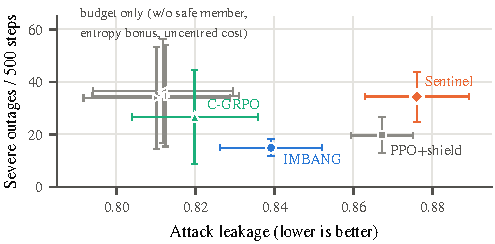
\includegraphics[width=\columnwidth]{figures/tradeoff.pdf}
\caption{Severe outages against attack leakage (Protocol~B, eight scenarios, 95\% confidence intervals over ten seeds). Only IMBANG reduces both relative to Sentinel.}
\label{fig:tradeoff}
\end{figure}

\textbf{Deployment and limitations.} The deployed actor has 5{,}447 parameters (21.8\,kB). On one 2.1\,GHz core, a decision including shielding takes 0.24\,ms, far below sub-second control windows. The study has four limitations:
\begin{itemize}
\item On zero-shot ICMP floods, IMBANG incurs more severe outages than Sentinel (18.0 against 4.6, not significant); an operator applying Sentinel's ICMP constants every ten windows reduces this to 2.1 at 90\% recognition accuracy.
\item IMBANG does not surpass Constrained GRPO on the composite score; its advantage lies in meeting the outage budget reliably and in fewer outages.
\item Prop.~\ref{prop:safe} assumes congestion set by the offered load; filtering upstream of the bottleneck would need a congestion-aware safe direction.
\item All results come from simulation.
\end{itemize}

\textbf{Why one member suffices.} Fig.~\ref{fig:dyn} shows that the multiplier is not the bottleneck: without a safe-side member, $\lambda$ grows steadily while the outage rate barely moves, because most groups contain no member that avoids the outage. One guaranteed no-less-safe member gives the constraint a direction, so IMBANG meets the budget early with $\lambda$ almost constant. It replaces one of the eight members, so an iteration costs no more.

\textbf{Interpretability.} Depth-4 decision trees distilled from the final policies reproduce the filtering focus with 99.8\% held-out accuracy and the threshold and drop rate with mean absolute errors of 0.013 and 0.017. Behind the same shield they match the neural policy's validation score, so operators can audit or replace the network. The certified shield tuning is equally readable: it lowered the PanicGuard utilisation gate from 0.60 to 0.52 on average.

% ===========================================================================
\section{Conclusion}
% ===========================================================================
Group-relative training erases any safety cost that a whole group shares. IMBANG restores it with one guaranteed safe-side member per group, outperforming Sentinel and more than halving its severe outages; validation on real 5G traffic is future work.

\bibliographystyle{IEEEtran}
\bibliography{refs}

\end{document}
